\documentclass{article}
\usepackage{amsmath}
\usepackage{graphicx}
\usepackage[margin=1in]{geometry}

\title{ Aerial Alumni \\ 2015  VWCC AUTONOMOUS ROBOTICS COMPETITION }
\author{ Jason Doyle \\ B.S. Electrical Engineering \\ VPI \& SU \and Phillip Benzinger \\ B.S. Computer Science \\ Liberty University }

\date{ \today }

\begin{document}

\maketitle

\clearpage

\tableofcontents
\listoffigures
\clearpage

\section{Executive Summary}

	The problem is to develop an autonomous robot to complete four trials set by Virginia Western Community College (VWCC). An autonomous air vehicle (AAV) was chosen to complete the trials for its challenge of use over a ground vehicle. The size of the robot can only be 8 in. x 12 in. x 10 in. high so a 250 size quad frame was chosen. 250 represents 250 mm diagonal distance between the center of two propellers. The frame was also chosen because it has a structure built under it, to allow all of the electronics to be mounted. Once the battery and flight controller were mounted to the frame it was realized that the frame would not be big enough. Since a camera, Raspberry Pi and Propeller micro controller still needed to be mounted another plate would need to be designed and built. 
	
	Size was a reoccurring issue with this design, because it needs to fly nothing could be mounted under the propellers. The original Propeller chip that was being used was mounted on a breadboard that took up the whole bottom plate. Since the Raspberry Pi also needed to be mounted to that plate a smaller solution was needed. The Propeller Hat was used to solve this problem it is a small board that is designed to mount on the top of the Raspberry Pi. The Propeller Hat has a small breadboard mounted to the top allowing wires to be easily connected, because of the height of the breadboard and wires coming out of it the board could not be mounted on top of the Raspberry Pi. There is enough space to mount the Propeller Hat next to the Raspberry Pi. The necessary wires are run from the Raspberry Pi to the Propeller Hat for communication and power. Size wasn't the only issue there were also several software issues.
	
	There were compatibility issues with Raspberry Pi's operating system and the required software. The software required to program the Propeller chip requires QT5 which only runs on Raspian Jessie the new version of Raspberry Pi's OS. OpenCV the computer vision library that is being used to find the red boxes didn't run on the new OS. Since it is more important for the OpenCV library to run on the Raspberry Pi than be able to program the Propeller chip the old OS Raspian Wheezy needed to be reinstalled. The Propeller software also had issues with the laptop but that has been solved with a virtual machine.

	There have been several issues with hardware and programs that have been solved not many with the software itself because at this point still needs a lot of work. The box detection software has been written and is working well but the flight software and communication software still need to be written and put together. In the future developing a flight controller that can communicate directly with the Raspberry Pi would add a lot of improvements. The improved flight controller would also cut down on weight and space.


\clearpage

\section{Bill of Materials}

	\begin{tabular}{ l l l c r r }
		\textbf{Item} & \textbf{Item Num.} & \textbf{Store} & \textbf{Qty} & \textbf{Unit Price} & \textbf{Subtotal} \\ \hline
		Frame & 366000015-0 & Hobby King & 1 & \$19.99 & \$19.99 \\
		Motor CCW & 9536000002-0 & Hobby King & 2 & \$12.13 & \$24.26 \\
		Motor CW & 9536000001-0 & Hobby King & 2 & \$12.13 & \$24.26 \\
		Speed Controller & 9192000258-0 & Hobby King & 4 & \$12.99 & \$51.96 \\
		Power Distribution & 9171000530-0 & Hobby King & 1 & \$1.89 & \$1.89 \\
		Flight Controller & 9171000593-0 & Hobby King & 1 & \$24.99 & \$24.99 \\
		Gemfan Multirotor 10 Pair 6x4.5 Black & 329000381-0 & Hobby King & 1 & \$10.20 & \$10.20 \\
		Parallax Propeller Hat & 32230 & Parallax.com & 1 & \$24.95 & \$24.95 \\
		Electronic Mounting Plate & Custom Part & VWCC & 1 & TBD	& TBD \\
%		Standoffs & & & 8 & & \\
%		Wire & & & & & \\
%		Connectors & & & & & \\
%		Black Zip Ties & 0076328 & Lowes & 8 & X & X \\
%		Thread Locker & 24200 & Lowes & N/A & N/A & N/A \\
		\hline
		\multicolumn{6}{ r }{\textbf{\$182.50}} \\ 
%	\end{tabular}
%
%	\subsection{Spare Parts}	
%	\begin{tabular}{ l l l c r r }
		\multicolumn{6}{ l }{\textbf{Spare parts}} \\
		\hline
		\textbf{Item} & \textbf{Item Num.} & \textbf{Store} & \textbf{Qty} & \textbf{Price} & \textbf{Subtotal} \\ \hline
		Speed Controller & 9192000258-0 & Hobby King & 2 & \$12.99 & \$25.98 \\
		Electronic Mounting Plate & Custom Part & VWCC & 1 & TBD	& TBD \\
		\hline
		\multicolumn{6}{ r }{\textbf{\$25.98}} \\ 
				
		\multicolumn{6}{ l }{\textbf{Shipping Costs}} \\ \hline
		\textbf{Shipper} & \textbf{From} &  &  &  & \textbf{Cost} \\ \hline
		EMS Express & \multicolumn{4}{ l }{Hobby King Int.} & \$38.47 \\
		Swiss Post Direct & \multicolumn{4}{ l }{Hobby King Int.} & \$2.46 \\
		USPS Priority Mail & \multicolumn{4}{ l }{Parallax Inc.} & \$7.15 \\
		\hline
		\multicolumn{6}{ r }{\textbf{\$48.08}} \\
		\cline{6-6}
		\multicolumn{5}{ r }{\textbf{Grand Total:}}  & \textbf{\$256.56}\\ 
	\end{tabular}
	
%\section{Weight Budget}

%	\begin{tabular}{ l c r r r r }
%		\textbf{Item} & \textbf{Qty.} & \textbf{Unit Lift (g)} & \textbf{Unit Weight (g)}  %& \textbf{Total Lift (g)} & \textbf{Total Weight (g)}\\ \hline
%		Speed Controller & 9192000258-0 & Hobby King & 2 & \$12.99 & \$25.98 \\
%		\hline
%		\multicolumn{6}{ r }{\textbf{\$000.00}} \\ 		
%		\multicolumn{6}{ l }{\textbf{Shipping Costs}} \\ \hline
%		\textbf{Shipper} & \textbf{From} &  &  &  & \textbf{Cost} \\ \hline
%		EMS Express & \multicolumn{4}{ l }{Hobby King Int.} & \$38.47 \\
%		Swiss Post Direct & \multicolumn{4}{ l }{Hobby King Int.} & \$2.46 \\
%		\hline
%		\multicolumn{6}{ r }{\textbf{\$000.00}} \\
%		\cline{4-6}
%		\multicolumn{5}{ r }{\textbf{Grand Total:}}  & \textbf{\$000.00}\\ 
%	\end{tabular}
	
\clearpage

\section{CAD Drawings}

\begin{figure}[h!]
\caption{Electronics plate}
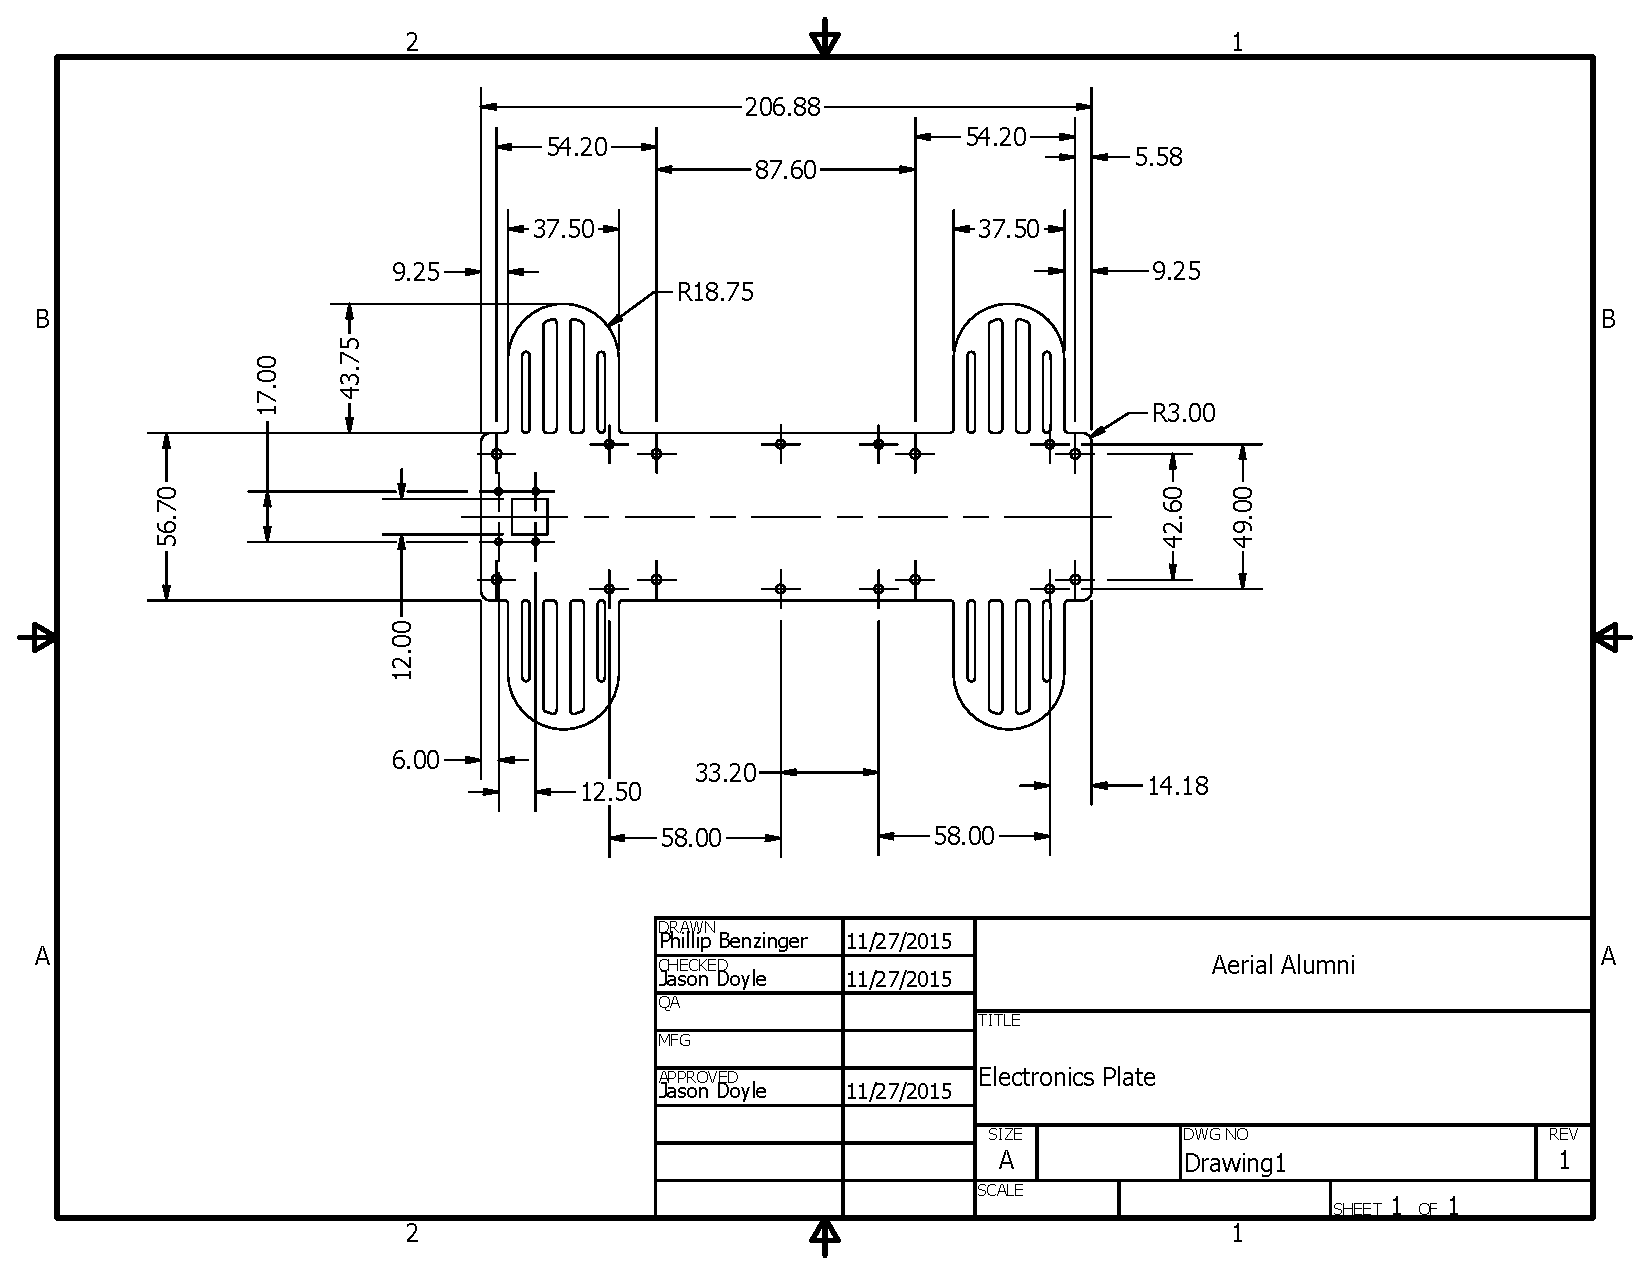
\includegraphics[scale=0.65, angle=90]{CAD.pdf}
\end{figure}

\begin{figure}[h]
\caption{Block Diagram}
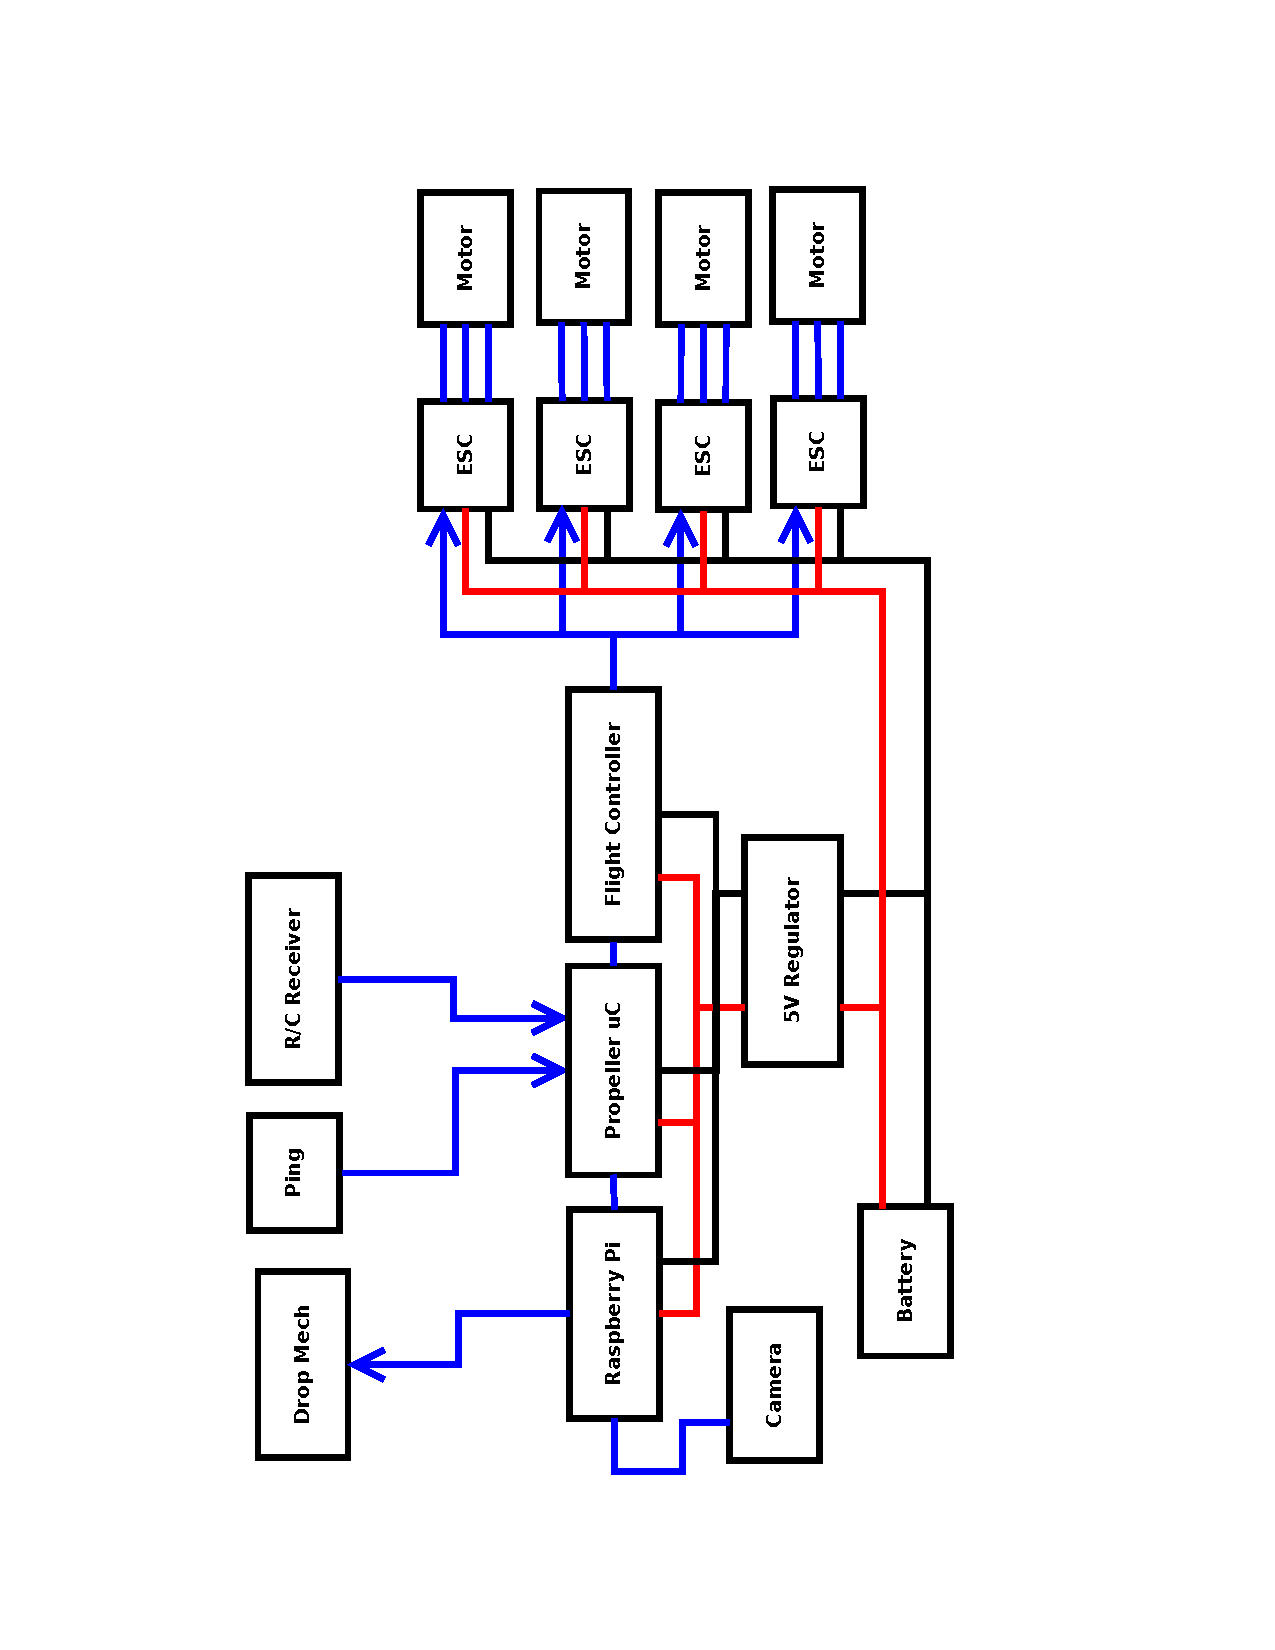
\includegraphics[width=\textwidth]{Block_Diagam_v2.pdf}
\end{figure}

\begin{figure}[h]
\caption{Propeller $\mu$C connections}
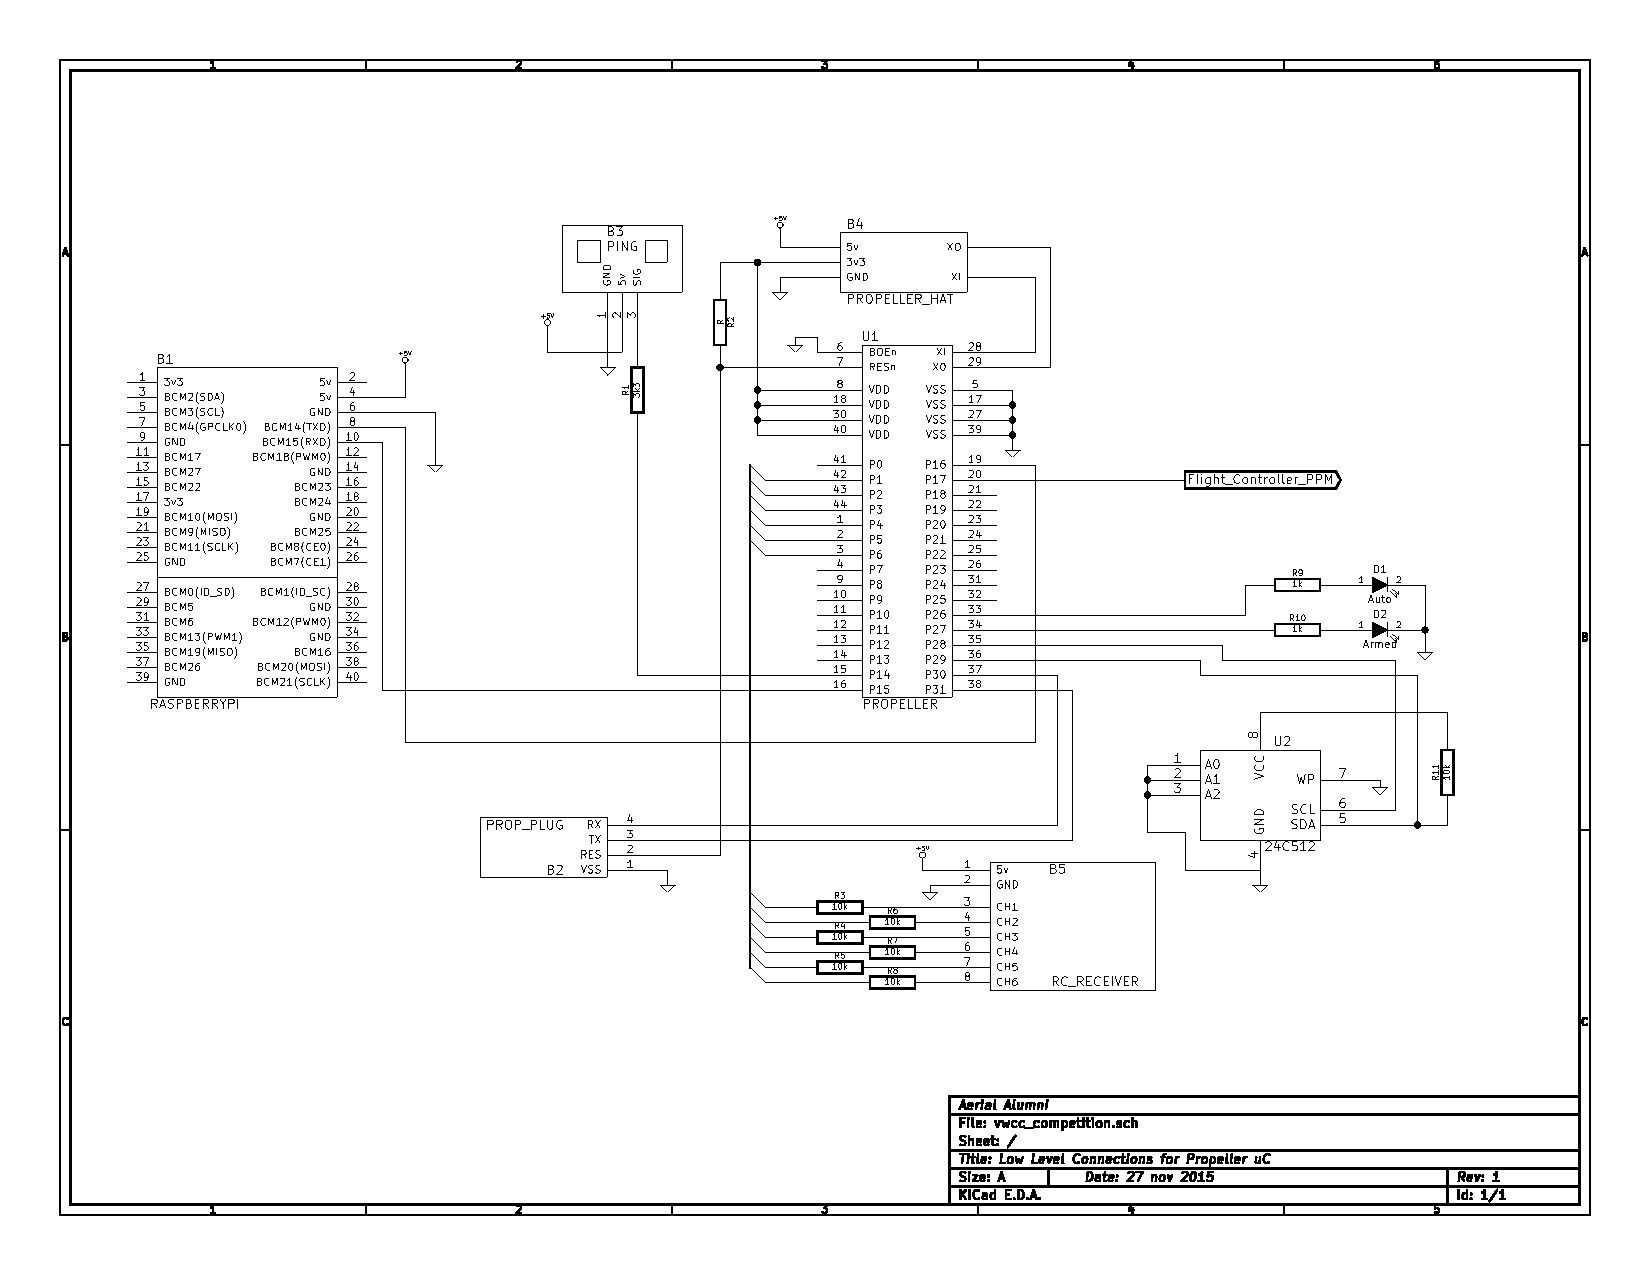
\includegraphics[height=\textwidth, angle=90]{vwcc_competition.pdf}
\end{figure}

\begin{figure}[h]
\caption{Autonomous and arming flight mode controls from radio controller.}
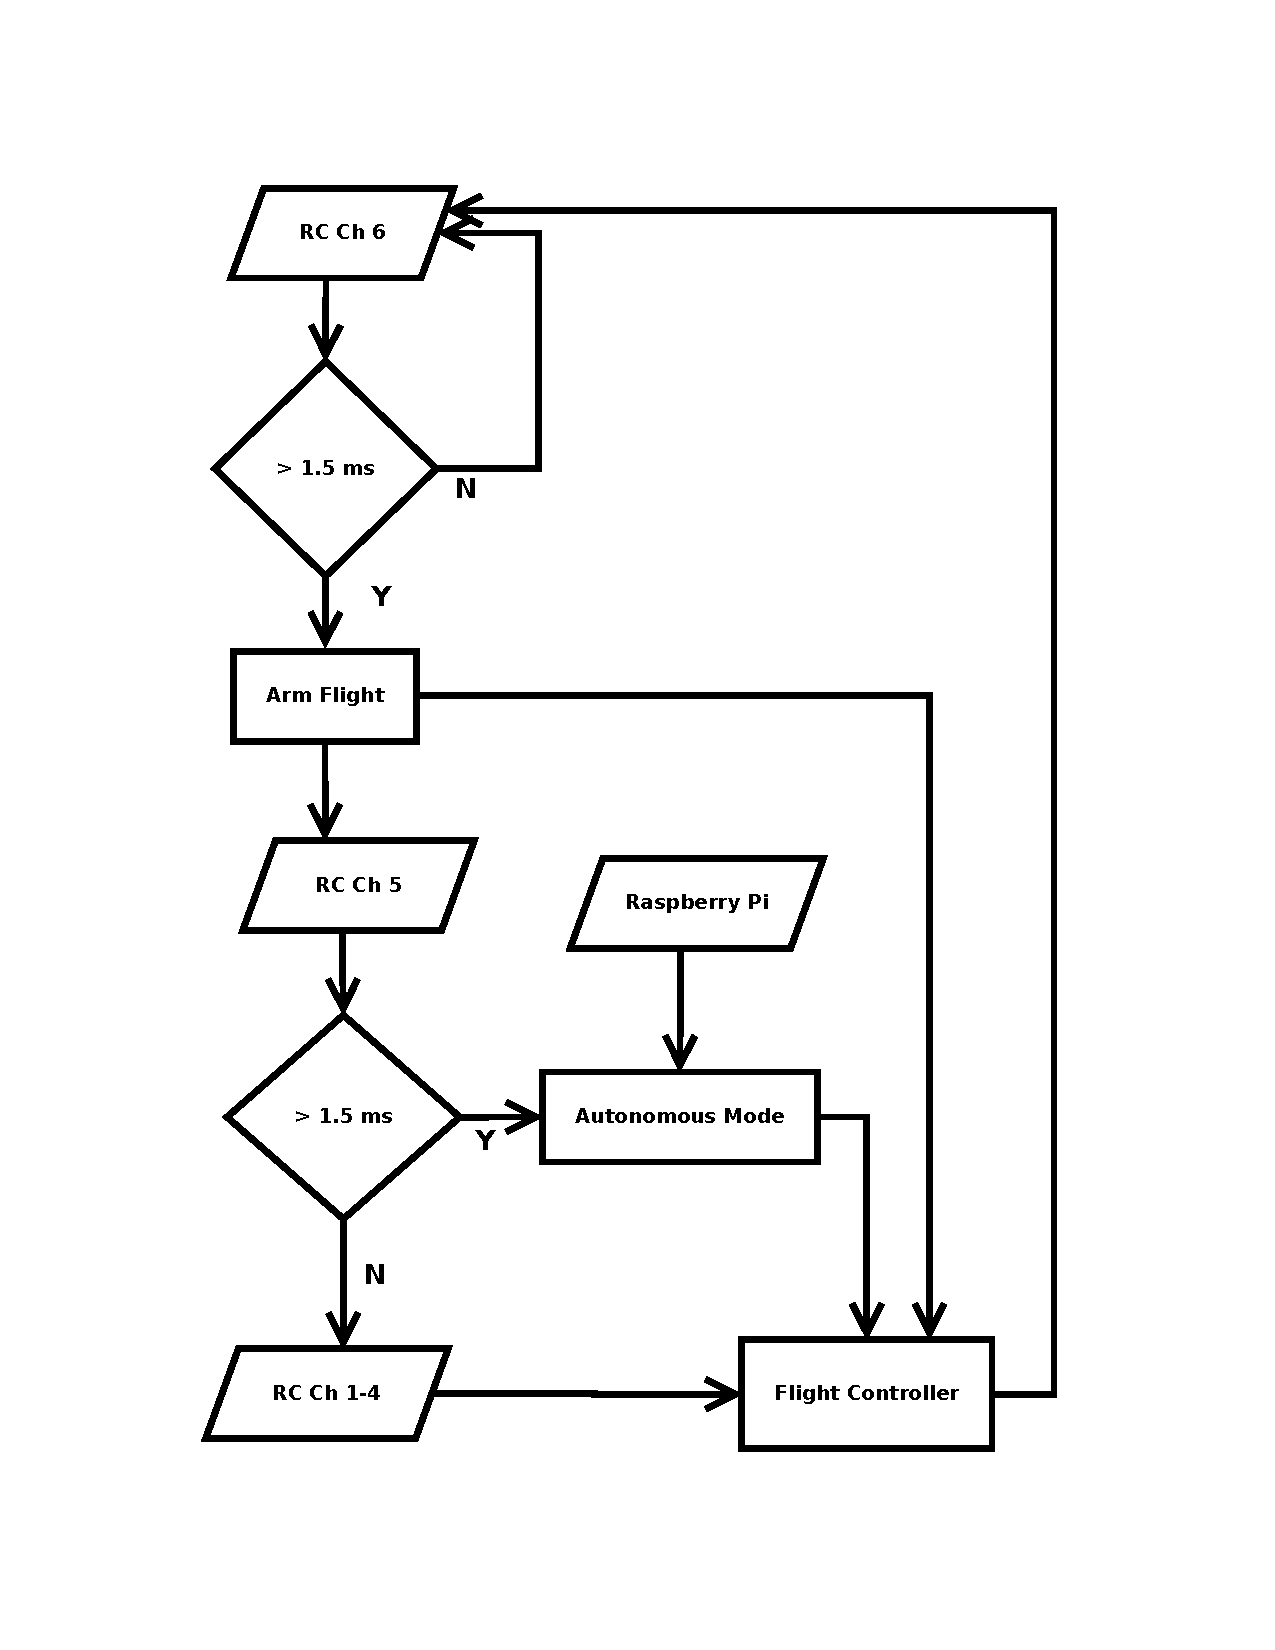
\includegraphics[width=\textwidth,]{Arm_auto.pdf}
\end{figure}

\begin{figure}[h]
\caption{Propeller $\mu$C flow chart.}
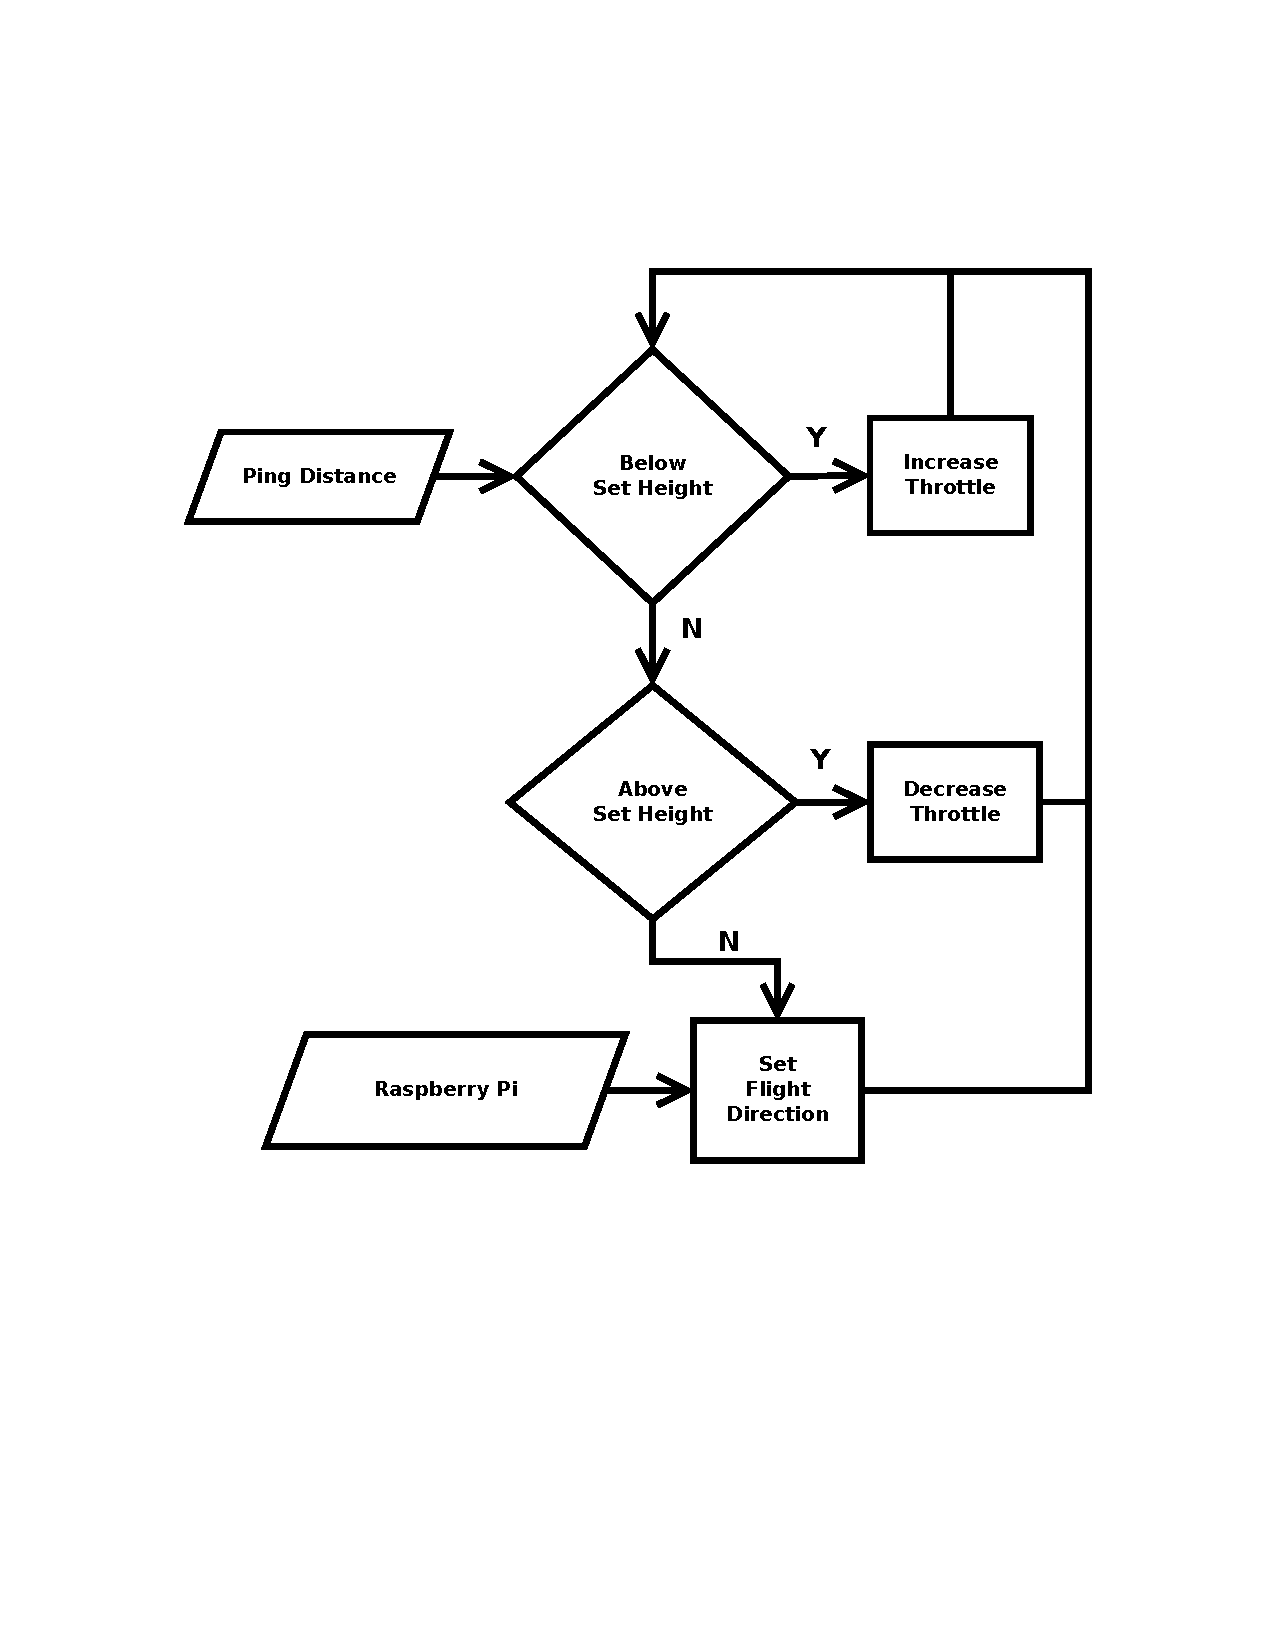
\includegraphics[width=\textwidth,]{Propeller_Flight.pdf}
\end{figure}

\begin{figure}[h]
\caption{Raspberry Pi flow chart.}
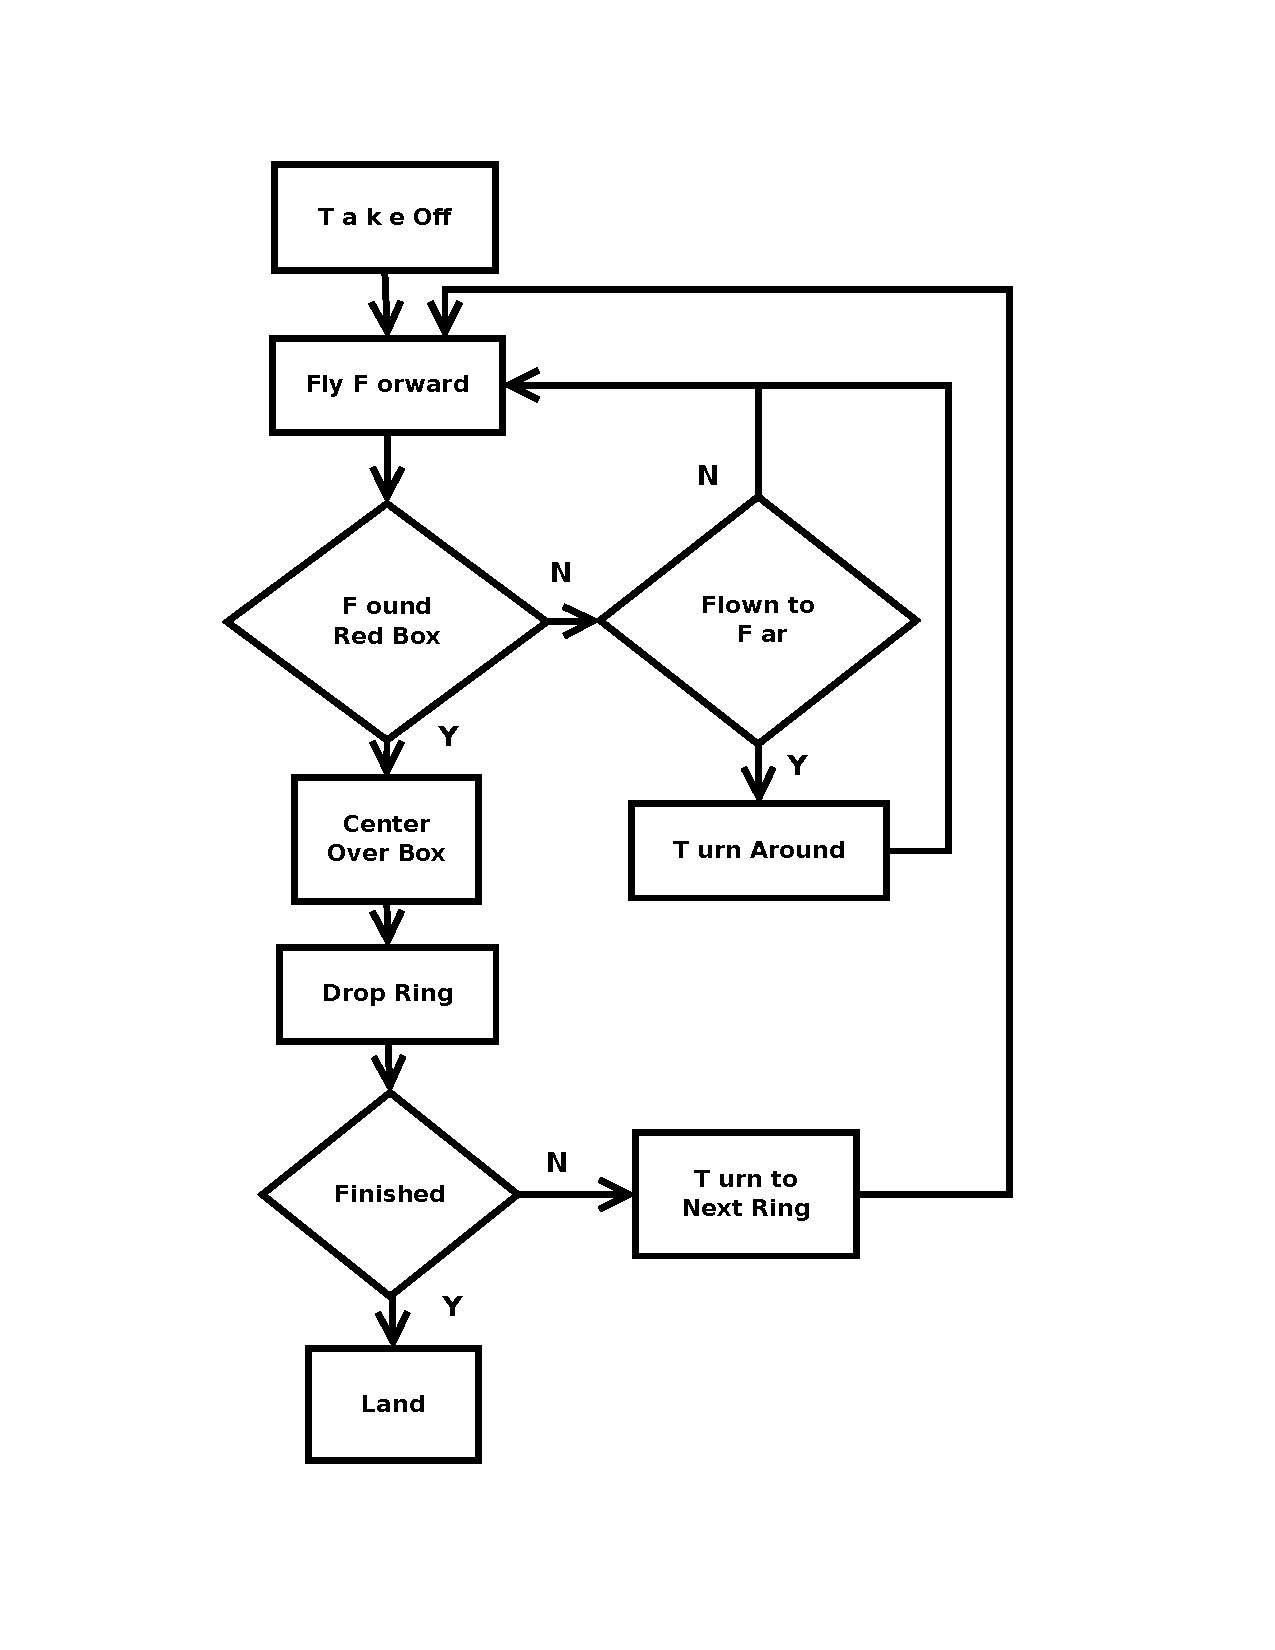
\includegraphics[width=\textwidth,]{raspberrypi.pdf}
\end{figure}

\end{document}